\section{Aufbau}
\label{sec:Aufbau}

\begin{figure}
	\centering
	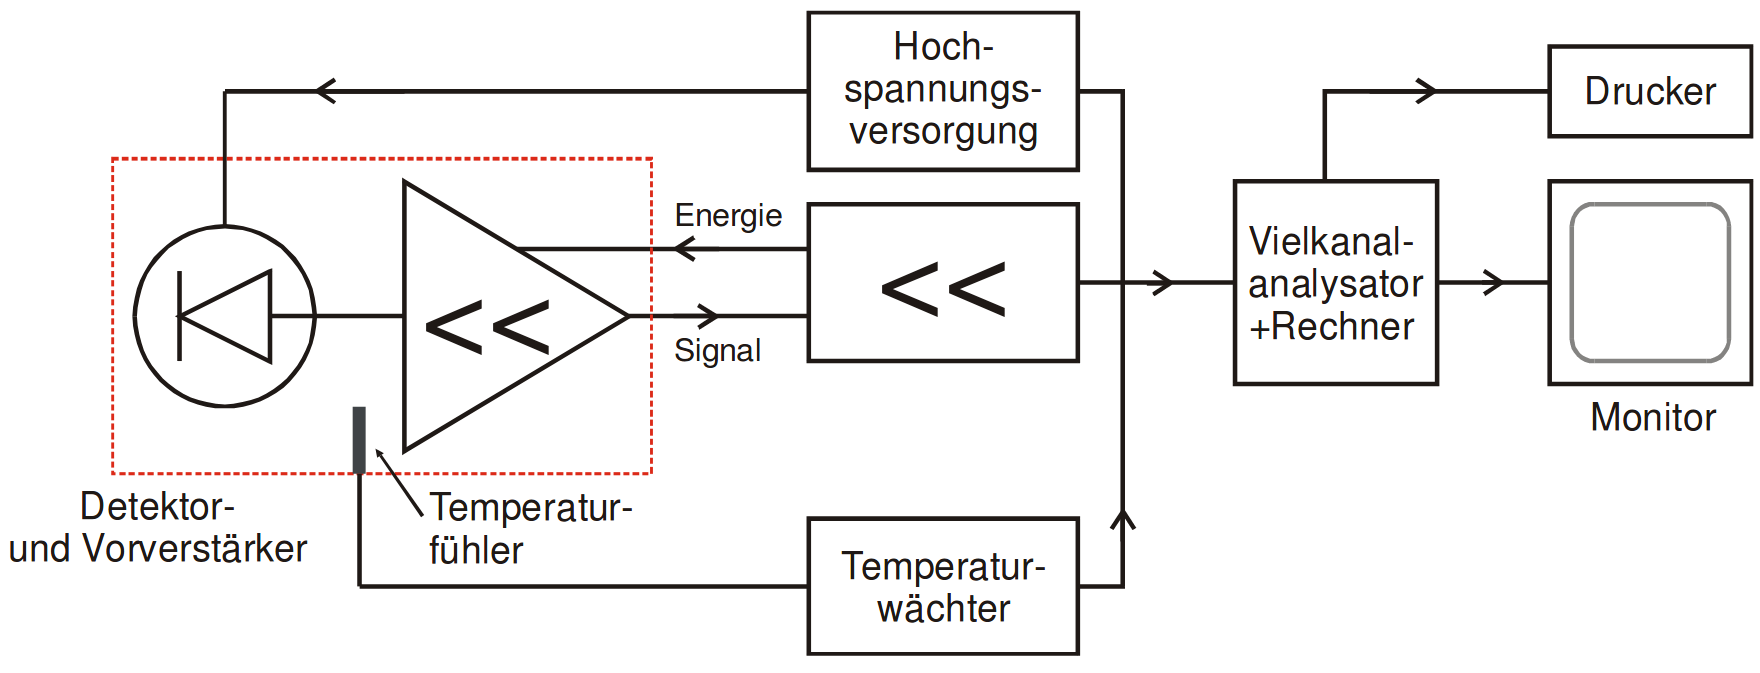
\includegraphics[width=\linewidth-100pt,height=\textheight-100pt,keepaspectratio]{content/Images/detektor.png}
    \caption{Der schematische Aufbau eines Germaniumdetektors  \cite{V18}.}
    \label{fif:spektrum}
\end{figure}

%bild vom aufbau einfügen
Der verwendete Germaniumdetektor ist zylindrisch und und besitzt eine koaxiale Bohrung in seinem Inneren. Die Oberfläche ist aufgrund von eindiffundiertem Lithium stark n-dotiert, die Oberfläche der Bohrung aufgrund einer Goldbedampfung stark p-dotiert. Die externe Sperrspannung wird an der Innen und Aussenseite angelegt. Das Detektormaterial wird durch eine Aluminiumschutzhaube geschützt, welche allerdings dafür sorgt, dass Gammaquanten mit Energien unterhalb von $\SI{40}{\kilo\electronvolt}$ nicht registriert werden können. Die Probe wird mehrere $\si{\centi\meter}$ oberhalb des Detektors in einer Halterung fixiert. Die im Detektor entstandenen Ladungsimpulse müssen nun in eine geeignete Messgröße umgewandelt werden. Hierzu gelangen die Impulse zunächst in einen Vorverstärker. In diesem wird eine Spannung erzeugt, welche proportional zu dem über die Zeit integrierten Strom ist. Damit die Spannung nach einem eingegangenen Impuls wieder auf Null zurückfällt und es zu keiner Spannungsaddition der Impulse kommt, muss sie nach dem Ende des Impulses wieder abfließen. Da ein parallel geschalteter Wiederstand jedoch zu verstärktem Rauschen führen würde wird eine optoelektronische Schaltung verwendet. Diese lässt den Strom abfließen, sobald die Spannung eine obere Schwelle überschreitet. Um Rauscheffekte zu minimieren werden sowohl Detektor als auch Vorverstärker mit flüssigem Stickstoff auf $\SI{77}{\kelvin}$ heruntergekühlt. Die Hochspannungsversorgung ist zudem an einen Temperaturwächter gekoppelt, da die anliegende Spannung bei höheren Temperaturen das Detektormaterial beschädigen würde. Da der Vorverstärker bei einem plötzlichen Spannungsabfall jedoch beschädigt werden würde ist ein RC-Glied mit großer Zeitkonstante zwischengeschaltet. Anschließend gelangt die Spannung über eine kapazitative Signalleitung mit niedriger Impedanz in den Hauptverstärker. Dieser verstärkt die Signale auf einen Spannungsbereich von $0 - \SI{10}{\volt}$. Es ist darauf zu achten, dass die Verstärkung zeitlich konstant bleibt und die Bandbreite des Verstärkers geeignet gewählt wird. Letzteres reduziert zusätzliches rauschen. Danach werden die Impulse in einem Analog zu Digital Konverter, kurz ADC, in digitale Signale umgewandelt. In diesem wird mithilfe der eingehenden Spannung ein Kondensator aufgeladen. Danach entlädt sich dieser wieder über eine Konstantstromquelle und die dafür benötigte Zeit wird mithilfe eines Quarzosszillators gemessen. Wenn am Kondensator wieder eine Spannung von Null anliegt wird die Zählung beendet und das ergebnis an einen Binärzähler weitergeleitet. Damit während des Entladevorgangs kein weiterer Impuls in den ADC gelangt wird dessen Eingang über eine integrierte Steuereinheit für die benötigte Zeit gesperrt. Diese liegt bei etwa $\SI{40}{\micro\second}$. Zusätzlich ist eine PUR-Schaltung vor den ADC geschaltet, welche diesen im Falle mehrerer Impulse in kurzer Zeit sperrt, da sich diese ansonsten zu einem großen Impuls addieren würden. Beide Effekte können durch Differenzierung zwischen der Messzeit, ohne die Totzeiten und der Echtzeit berücksichtigt werden. Zuletzt gelangen die Signale in einen Vielkanalanalysator. In diesem wird den Signale anhand ihrer Höhe, welche proportional zur Energie ist, eine Binärzahl zugeordnet. Wird nun ein Impuls registriert wird der Inhalt des Speichers der zugehörigen Binärzahl um Eins erhöht Der verwendete Detektor besitzt 8192 Kanäle. Nach der Messung erhält man das Spektrum des Strahlers.